\subsection{Photoionisation}

\begin{figure}[htbp]
    \centering
    \resizebox{\textwidth}{!}{
\begin{tikzpicture}[
  scale=0.62,
  well/.style      = {thick, black, line cap=round},
  ipline/.style    = {gray!70, thin},
  photonarr/.style = {photon,   line width=1.0pt, -{Stealth[length=5pt]}},
  elecarr/.style   = {electron, line width=1.1pt, -{Stealth[length=5pt]}},
  tick/.style      = {photon,   line width=1.0pt},
  panellabel/.style= {font=\small},
  regime/.style    = {font=\scriptsize, align=center, text width=2.8cm}
]

% étiquette -Ip (une seule fois, à gauche)
\node[font=\small] at (-2.65,-1) {$-I_p$};

% =====================================================================
% a) SINGLE-PHOTON  (xshift 0) : puits symétrique, flèche pleine
% Paramètre a = 0
% =====================================================================
\begin{scope}[xshift=0cm]
  \clip (-2.3,-2.05) rectangle (2.5,1.7);
  \draw[well] plot[domain=-2.5:-0.1, samples=50] (\x, {-1/(5*\x*\x) + 1});
  \draw[well] plot[domain=0.1:2.5, samples=50] (\x, {-1/(5*\x*\x) + 1});
  \draw[ipline] (-2.2,-1)--(2.2,-1);
  \draw[photonarr] (0,-1)--(0,1);
\end{scope}
\node[panellabel] at (-2.0,2.05) {a)};
\node[regime]     at (0,-2.75)   {single-photon\\ionization};

% =====================================================================
% b) ABOVE-THRESHOLD MPI  (x-shift 5) : même puits, flèche pointillée + rungs
% Paramètre a = 0
% =====================================================================
\begin{scope}[xshift=5cm]
  \clip (-2.3,-2.05) rectangle (2.5,1.7);
  \draw[well] plot[domain=-2.5:-0.1, samples=50] (\x, {-1/(5*\x*\x) + 1});
  \draw[well] plot[domain=0.1:2.5, samples=50] (\x, {-1/(5*\x*\x) + 1});
  \draw[ipline] (-2.2,-1)--(2.2,-1);
  % flèche pointillée
  \draw[photonarr] (0,-1.0)--(0,-0.5);
  \draw[photonarr] (0,-0.5)--(0,-0.0);
  \draw[photonarr] (0,0)--(0,0.5);
  \draw[photonarr] (0,0.5)--(0,1.0);
  

\end{scope}
\node[panellabel] at (3.0,2.05) {b)};
\node[regime]     at (5,-2.75)  {above-threshold\\multi-photon ionization};

% =====================================================================
% c) NON-ADIABATIC TUNNEL  (xshift 10) : barrière large, montée + tunnel
% Paramètre a = 0.1
% =====================================================================
\begin{scope}[xshift=10cm]
  \clip (-2.3,-2.05) rectangle (2.5,1.7);
  \draw[well] plot[domain=-2.5:-0.1, samples=50] (\x, {-1/(5*\x*\x) + 1 - 0.5*\x});
  \draw[well] plot[domain=0.1:2.5, samples=50] (\x, {-1/(5*\x*\x) + 1 - 0.5*\x});
  \draw[ipline] (-2.2,-1)--(2.2,-1);
  % montée multiphotonique (courte, jaune)
  \draw[photonarr] (0,-1.0)--(0,-0.5);
  \draw[photonarr] (0,-0.5)--(0,-0.0);
  % tunnel à travers la barrière (vert, sortie à droite)
  \draw[elecarr] (0,-0)--(2.60,-0);
\end{scope}
\node[panellabel] at (8.0,2.05)  {c)};
\node[regime]     at (10,-2.75)  {non-adiabatic\\tunnel ionization};

% =====================================================================
% d) ADIABATIC TUNNEL  (xshift 15) : barrière plus inclinée, tunnel à -Ip
% Paramètre a = 0.9
% =====================================================================
\begin{scope}[xshift=15cm]
  \clip (-2.3,-2.05) rectangle (2.5,1.7);
  \draw[well] plot[domain=-2.5:-0.1, samples=50] (\x, {-1/(5*\x*\x) + 1 - 1.9*\x});
  \draw[well] plot[domain=0.1:2.5, samples=50] (\x, {-1/(5*\x*\x) + 1 - 1.9*\x});
  \draw[ipline] (-2.2,-1)--(2.2,-1);
  % tunnel horizontal au niveau -Ip
  \draw[elecarr] (0,-1)--(2.25,-1);
\end{scope}
\node[panellabel] at (13.0,2.05) {d)};
\node[regime]     at (15,-2.75)  {adiabatic\\tunnel ionization};

% =====================================================================
% e) OVER-BARRIER  (xshift 20) : barrière abaissée sous -Ip, sortie libre
% Paramètre a = 1.6
% =====================================================================
\begin{scope}[xshift=20cm]
  \clip (-2.3,-2.05) rectangle (2.5,1.7);
  \draw[well] plot[domain=-2.5:-0.1, samples=50] (\x, {-1/(5*\x*\x) + 1 - 2.8*\x});
  \draw[well] plot[domain=0.1:2.5, samples=50] (\x, {-1/(5*\x*\x) + 1 - 2.8*\x});
  \draw[ipline] (-2.2,-1)--(2.2,-1);
  % l'électron passe au-dessus de la barrière supprimée
  \draw[elecarr] (0.0,-1)--(2.30,-1);
\end{scope}
\node[panellabel] at (18.0,2.05) {e)};
\node[regime]     at (20,-2.75)  {over-barrier\\ionization};

\end{tikzpicture}
}
    \caption{Illustration des différents régimes d'ionisation.}
    \label{fig:regimes_ionisation}
\end{figure}

Une forte focalisation conduit à une intensité optique élevée dans le matériau. Cette forte concentration de photons au même endroit augmente la probabilité d'ionisation multiphotonique, un effet non-linéaire~\cite{mao2004}. Plus le champ est intense, plus le potentiel liant l'électron à l'ion est déformé. Au-delà d'un certain seuil d'intensité, la barrière prend une forme triangulaire et devient suffisamment fine pour permettre l'ionisation par effet tunnel. Le paramètre de Keldysh a été introduit pour distinguer entre le régime où domine l'ionisation multiphotonique et celui où domine l'ionisation par effet tunnel~\cite{mao2004}.

Dans le modèle semi-classique, un électron s'échappe à travers une barrière de largeur $l = U_i/e\mathcal{E}$ avec une vitesse $v = \sqrt{2U_i/m}$. Le temps nécessaire pour traverser cette distance est :
\begin{equation}
\tau_{\text{tun}} = \frac{l}{v} = \frac{U_i/e\mathcal{E}}{\sqrt{2U_i/m}} = \frac{\sqrt{2m U_i}}{e\mathcal{E}}
\end{equation}

Le temps caractéristique pendant lequel l'ionisation par effet tunnel peut se produire est donné par $\tau \approx 1/\omega_0$. Le rapport de ces temps est alors :
\begin{equation}
\gamma = \frac{\tau_{\text{tun}}}{\tau} = \omega_0\frac{\sqrt{2m U_i}}{e\mathcal{E}}
\end{equation}

Si le rapport $\gamma \ll 1$, cela signifie que le temps de traversée par effet tunnel est très court comparé au temps d'ionisation. L'effet tunnel est instantané à l'échelle du cycle laser. Le champ se comporte comme un champ quasi-statique. Inversement, si $\gamma \gg 1$, le champ oscille trop rapidement pour permettre à l'électron de traverser la barrière par effet tunnel, l'ionisation nécessite alors une absorption multiphotonique~\cite{bulgakova2010}.

Le taux de photoionisation de Keldysh est défini comme suit :
\begin{equation}
W_{PI}(|\mathcal{E}|) = \frac{2\omega_0}{9\pi}\bigg(\frac{\omega_0m}{\hbar\sqrt{\gamma_1}}\bigg)^{\frac{3}{2}}Q(\gamma,x)\exp(-\alpha\lceil x+1\rceil)
\end{equation}

Avec $\gamma_1 = \frac{\gamma^2}{1+\gamma^2}$, $\gamma_2 = \frac{1}{1+\gamma^2}$ et $x = \frac{2}{\pi}\frac{U_iE(\gamma_2)}{\hbar\omega_0\sqrt{\gamma_1}}$
\begin{equation}
Q(\gamma,x) = \frac{\pi}{2K(\gamma_2)}\sum^\infty_{n=0}\exp \bigg(-n\pi\frac{K(\gamma_1)-E(\gamma_1)}{E(\gamma_2)}\bigg)\Phi\bigg(\frac{\pi}{2}\sqrt{\frac{n+2\lceil x + 1\rceil-2x}{K(\gamma_2)E(\gamma_2)}}\bigg)
\end{equation}

$\Phi$ est la fonction de Dawson $\Phi(z) = e^{-z^2}\int^z_0e^{y^2}dy$ et $K$ et $E$ sont les intégrales elliptiques complètes respectivement de première et deuxième espèce, avec le paramètre $m = k^2$
\begin{align}
K(m) &= \int_0^{\pi/2} [1 - m \sin(t)^2]^{-1/2} dt \\
E(m) &= \int_0^{\pi/2} [1 - m \sin(t)^2]^{1/2} dt
\end{align}

Comme observé dans la référence~\cite{PhysRevB.71.125435}, la filamentation dans la silice fondue se produit typiquement à des intensités autour de $5 \times 10^{13} \text{ W/cm}^2$, où l'ionisation multiphotonique et par effet tunnel contribuent toutes deux de manière significative.

\begin{figure}[htbp]
    \centering
    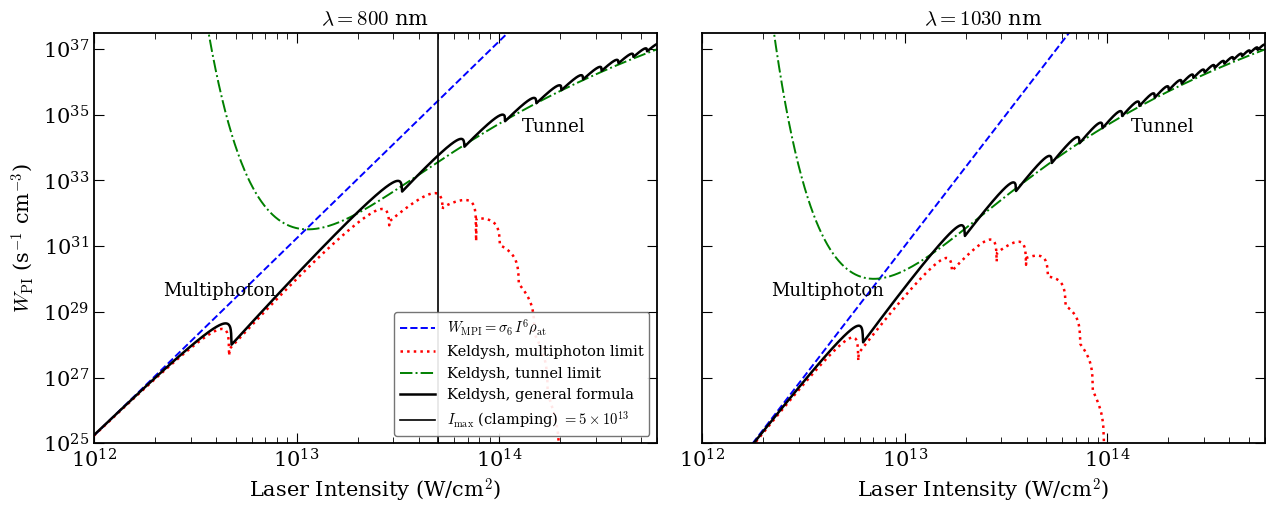
\includegraphics[width=1\linewidth]{sections/téléchargement.png}
    \caption{Le taux de photoionisation $W_{\text{PI}}$ dans la silice fondue ($U_i = 9 \text{ eV}$) est tracé en fonction de l'intensité laser pour $\lambda = 800 \text{ nm}$ et $\lambda = 1030 \text{ nm}$. La ligne solide noire représente la formule générale complète de Keldysh, tandis que les lignes pointillées rouges et tiret-point vert montrent ses asymptotes analytiques exactes pour les limites multiphotonique ($\gamma \gg 1$) et tunnel ($\gamma \ll 1$) respectivement. La ligne bleue en pointillés correspond à la loi MPI perturbative standard ($W_{\text{MPI}} = \sigma_K I^K \rho_{\text{at}}$). La ligne grise verticale indique le niveau typique d'intensité de clampage ($\sim 5 \times 10^{13} \text{ W/cm}^2$) atteint dans les simulations de filamentation à 800 nm.}
    \label{fig:placeholder}
\end{figure}
